\documentclass[11pt]{article}

\usepackage[T1]{fontenc}
\usepackage[utf8]{inputenc}
\usepackage{lmodern}
\usepackage{microtype}
\usepackage[margin=1in]{geometry}
\usepackage{amsmath,amssymb}
\usepackage{graphicx}
\usepackage{booktabs}
\usepackage{tabularx}
\usepackage{xcolor}
\usepackage{enumitem}
\usepackage{algorithm}
\usepackage{algpseudocode}
\usepackage[hidelinks]{hyperref}
\usepackage[numbers,sort&compress]{natbib}

\definecolor{violet}{HTML}{6250D6}
\newcommand{\pass}{\textsc{pass}}
\newcommand{\fail}{\textsc{fail}}
\newcommand{\incon}{\textsc{inconclusive}}
\setlist{itemsep=2pt,topsep=4pt}

\title{\textbf{Self-Improving MCP}\\[4pt]\large Evidence-Gated Evolution of Tool Interfaces for AI Agents}
\author{Shubham Singh}
\date{November 2026}

\begin{document}
\maketitle

\begin{abstract}
Agents choose tools from what a Model Context Protocol (MCP) server tells them. When tool descriptions are missing, vague or
overlapping, agents pick the wrong tool or build arguments that cannot run, and server authors rarely see it. Letting a language
model rewrite tool descriptions is easy; knowing whether a rewrite helps is not, and an unchecked rewrite measurably hurt tool
selection in our early experiments. We present \emph{Self-Improving MCP}, a runtime that places a transparent proxy in front of
any MCP server, records how agents use it, learns description changes from the agent's mistakes on one set of labeled tasks, and
ships a change only through a \emph{selection gate} that judges it on sealed tasks the learner never saw. A pick counts as correct
only if the tool is right (or an equivalent) \emph{and} its arguments are valid for the tool actually called; disputed tasks are
re-asked and counted only when decisive; a one-sided exact sign test with a zero-regression rule decides. On five domains of
MCPToolBench++ with \texttt{gpt-4.1-mini} as the agent, the gate failed every deliberately harmful change with exactly the
predicted number of broken tasks and never reported a difference for an empty change. For a server shipped without
descriptions, the loop learned descriptions that fixed 17 sealed tasks and broke none ($p<10^{-4}$), outperforming the server's
own descriptions (15 fixed, 2 broken). Where servers already document their tools, it found nothing to ship, and we show that
this is because that agent rarely depends on descriptions: it scores the same or better without them on four of five domains.
Open-weight agents behave differently: removing descriptions costs \texttt{gpt-oss-20b} 8 of 73 File System tasks and
\texttt{gpt-oss-120b} 6. We argue that strong agents make poor, short-lived test subjects (too few mistakes to measure, and
indifference to the interface being improved) and adopt a small open agent as the primary testbed. We also report the
measurement errors that, uncorrected, had produced a spurious +8.6-point gain.
\end{abstract}

\section{Introduction}

The Model Context Protocol~\cite{mcp2024} standardises how an agent discovers and calls tools: a server lists tools with a name,
a natural-language description and a JSON input schema, and the agent decides which to call. The description is therefore part of
the interface, and it is written once, by a person, without feedback from the agents that read it. Prior work shows that
documentation quality strongly affects tool use~\cite{hsieh2023tooldoc,yuan2024easytool}, and that language models can optimise
their own prompts~\cite{zhou2022ape,yang2023opro,khattab2023dspy}. Combining the two suggests an obvious product: let a model
rewrite tool descriptions from observed failures.

The obvious product is unsafe. In an early version of this work an ungated rewrite lowered tool-selection accuracy on held-out
tasks from 0.877 to 0.712. The hard part is not proposing a change; it is deciding, with evidence an operator can trust, whether
the change helps the agent \emph{as production would experience it}. This paper is about that decision.

\paragraph{Contributions.}
\begin{itemize}
  \item A runtime architecture that separates a deterministic, model-free hot path (proxy, recording, versioned
        \emph{overlays}, hot reload) from an offline improvement loop (Section~\ref{sec:system}).
  \item A \emph{selection gate} that scores executable correctness, controls for model non-determinism, and makes regressions
        fatal (Section~\ref{sec:gate}).
  \item An evidence-driven improver with guards against leakage and a pruning step that stops refinement from diverging
        (Section~\ref{sec:improver}).
  \item An evaluation design with known-answer controls and a simulation of undocumented servers, applied to five
        MCPToolBench++ domains~\cite{mcptoolbenchpp}, including the measurement errors we found in our own earlier results
        (Sections~\ref{sec:eval}--\ref{sec:lessons}).
\end{itemize}

\section{Background and related work}

\paragraph{Tool use.} Language models learn to call tools from demonstrations or self-supervision~\cite{schick2023toolformer},
can be specialised for large API collections~\cite{patil2023gorilla,qin2023toolllm}, and benefit from tool documentation
rather than many demonstrations~\cite{hsieh2023tooldoc}; concise, unified tool instructions improve agents~\cite{yuan2024easytool}.
These works change the \emph{model} or rewrite documentation offline; we change the \emph{interface} a deployed server presents,
continuously and behind a gate.

\paragraph{Prompt optimisation.} APE~\cite{zhou2022ape}, OPRO~\cite{yang2023opro} and DSPy~\cite{khattab2023dspy} search over
instructions using a score on training examples. Our improver is similar in spirit, but the score that decides shipping is
computed on a sealed split with paired statistics, and the object being optimised is shared by every agent that uses the server,
so a regression is costly.

\paragraph{Controlled experiments.} Our gate borrows from online experimentation~\cite{kohavi2020trustworthy}: paired comparison
on the same units, pre-registered decision rules, A/A tests to validate the instrument. With paired binary outcomes, the exact
sign test on discordant pairs is the exact form of McNemar's test~\cite{mcnemar1947}.

\section{System}\label{sec:system}

\begin{figure}[t]
  \centering
  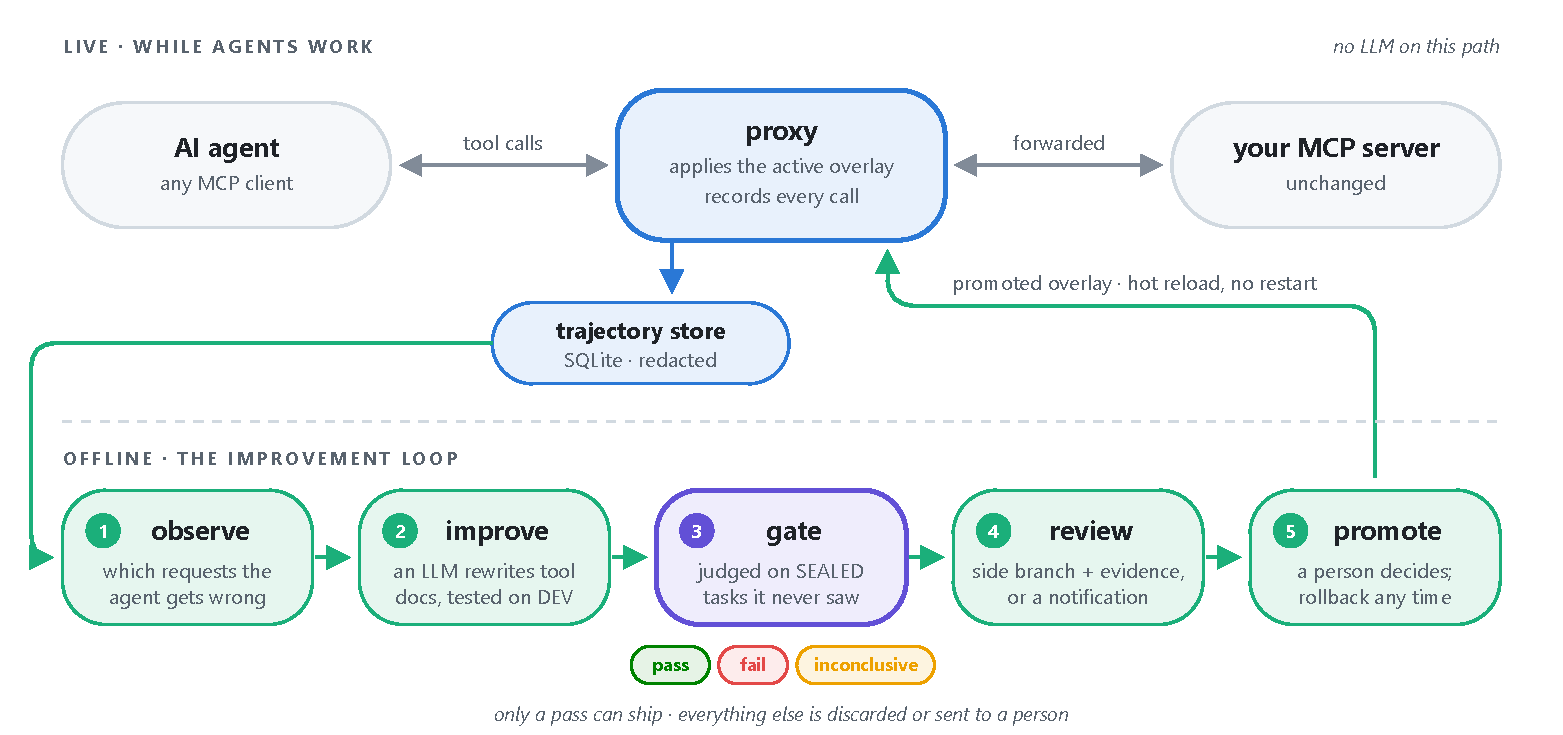
\includegraphics[width=\linewidth]{figures/how-it-works.pdf}
  \caption{Architecture. Live, a proxy sits between any MCP client and the unchanged server, applies the active overlay and
  records every call. Offline, the loop observes, improves on DEV tasks, judges on SEALED tasks, and hands the result to a
  person; a promoted overlay is hot-reloaded without restarting the proxy.}
  \label{fig:arch}
\end{figure}

\paragraph{Overlays.} A change is an \emph{overlay}, a versioned JSON document the proxy applies on top of the real server. It
can replace or hide a tool's advertised description or schema, route a call to another tool (or deny it), cache idempotent
results, and define composed tools. A single function computes the tool list an agent sees under an overlay; the proxy serves
it and the gate measures with it, so what is measured is what is served.

\paragraph{Hot path.} The proxy (Go, official MCP SDK) forwards calls and records, per call, the tool, redacted arguments and
their hash, a result summary, error flag and latency in SQLite. OpenTelemetry~\cite{otel} spans carry the session, the active
overlay version and, for routed calls, the tool originally requested. No language model is ever invoked on this path.

\paragraph{Promotion and rollback.} Promotion moves an \emph{active} pointer in the store. The proxy polls it, validates the
new overlay against the live tool list, swaps the served tools in place and notifies clients; an invalid overlay is refused while
the last good one keeps serving. Rolling back to the plain server is the same operation.

\paragraph{Executable routes.} A route renames a call but not its arguments. A route whose target requires an argument the source
does not take, or that types a shared argument differently, is rejected by both the proxy and the gate before any measurement.

\section{The selection gate}\label{sec:gate}

\begin{figure}[t]
  \centering
  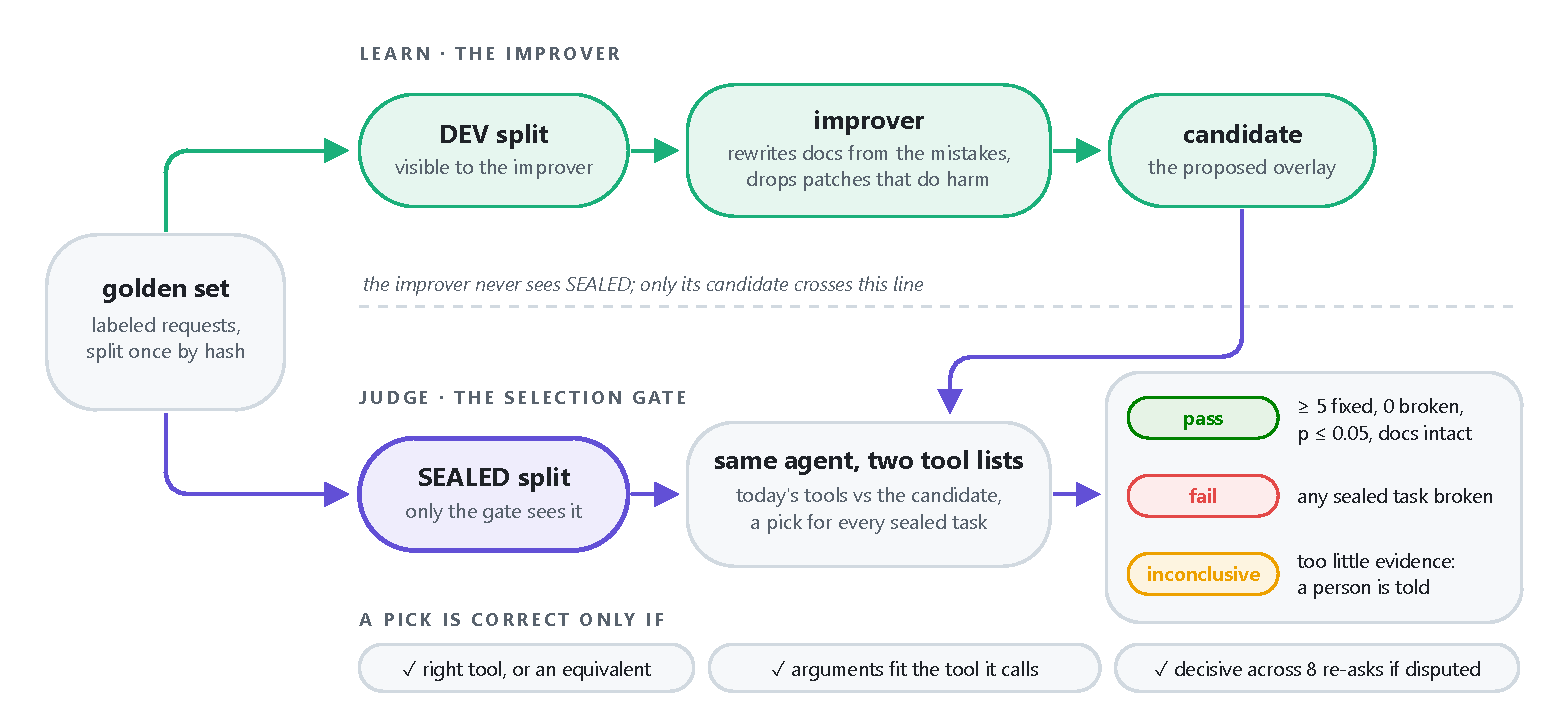
\includegraphics[width=\linewidth]{figures/gate.pdf}
  \caption{The gate. A golden set is split once into DEV (visible to the improver) and SEALED (visible only to the gate). The
  same agent picks a tool for every sealed task under today's tools and under the candidate.}
  \label{fig:gate}
\end{figure}

\paragraph{Correctness.} Let $T$ be the sealed tasks. For task $t$ the label is a tool $e_t$ with an equivalence set $E_t \ni e_t$
(tools that perform the same action, e.g.\ on a sibling server). Under arm $a\in\{B,C\}$ (baseline, candidate) the agent returns a
tool $\pi_a(t)$ and arguments $x_a(t)$; routing maps the call to $\rho_a(\pi_a(t))$. The task is correct under $a$ iff
\begin{equation}
c_a(t) = \mathbb{1}\big[\rho_a(\pi_a(t)) \in E_t \;\wedge\; x_a(t) \models \mathrm{schema}(\rho_a(\pi_a(t))) \;\wedge\; \neg\,\mathrm{denied}_a(t)\big].
\end{equation}
Requiring schema validity against the tool \emph{actually called} is what exposes routes that rename a call into a tool that
cannot accept it.

\paragraph{Non-determinism.} Hosted models are not deterministic at temperature 0: the same harmless change once moved a
borderline task and was falsely failed. Every task where $c_B(t)\neq c_C(t)$ is re-asked $k=8$ more times per arm. With $r_a(t)$
the fraction of correct votes, a task is \emph{fixed} if $r_C\ge 0.75$ and $r_B\le 0.25$, \emph{broken} in the mirror case, and
\emph{unstable} otherwise; unstable tasks are reported and excluded.

\paragraph{Decision.} With $F$ fixed and $K$ broken tasks, the one-sided exact sign test gives
\begin{equation}
p = \sum_{i=F}^{F+K} \binom{F+K}{i} 2^{-(F+K)}.
\end{equation}
In order: fewer than 30 sealed tasks or more than 5\% selector errors $\Rightarrow$ \incon; $K>K_{\max}$ (default 0) $\Rightarrow$
\fail; $F=0$ $\Rightarrow$ \incon; $p\le\alpha$ (0.05) $\Rightarrow$ \pass; otherwise \incon. With $K=0$ the smallest passing $F$
is $\lceil\log_2(1/\alpha)\rceil = 5$. The decision records the \emph{headroom} $|T|-\sum_t c_B(t)$; below 5 no candidate can pass,
and the gate says so rather than blaming the candidate.

\paragraph{Retention.} Selection accuracy cannot see information an agent needs \emph{after} choosing (result format, limits,
side effects). For every changed description, a judge checks each sentence of the old text (3 votes): is it needed after
choosing, and does the new text still state it? A loss turns \pass{} into \incon{} unless a person accepts it.

\paragraph{Shipping.} A \pass{} becomes a local branch with the overlay, the evidence and a pull-request text that shows new
descriptions verbatim and flags URLs or authority wording; nothing is pushed. \fail{} and \incon{} produce a notification.

\section{The improver}\label{sec:improver}

\begin{algorithm}[t]
\caption{Evidence-driven improvement on DEV}\label{alg:improve}
\begin{algorithmic}[1]
\State $R_0 \gets$ run agent on DEV under current overlay; \textbf{abort} if $>5\%$ calls failed
\State $M \gets$ group wrong outcomes of $R_0$ by (expected, observed)
\For{round $r = 1..3$}
  \State $P \gets$ \textsc{Propose}(tools as the agent sees them incl.\ parameters, $M$, feedback)
  \State drop patches for unknown tools, empty text, text copying $\ge 8$ words of a DEV request, hiding all tools
  \State $R \gets$ run agent on DEV with $P$
  \State $H \gets \{\tau\in P : \#\text{broken tasks involving }\tau > \#\text{fixed tasks involving }\tau\}$
  \If{$0<|H|<|P|$ \textbf{and} score$(P\setminus H) >$ score$(P)$} \State $P \gets P\setminus H$ \EndIf
  \State record round; feedback $\gets$ fixed, broken, still wrong, pruned
\EndFor
\State \Return best round if it beats $R_0$ by $\ge 2$ tasks, else nothing
\end{algorithmic}
\end{algorithm}

The improver (Algorithm~\ref{alg:improve}) sees what the agent sees: every tool's name, a compact parameter list and its
description, plus the requests the agent got wrong on DEV, grouped by pattern. It proposes description patches or hides a tool
marked deprecated; it never proposes routes, because a route cannot repair arguments built for the wrong tool. A task
``involves'' a patched tool if that tool is its label, an equivalent, or the tool served before or after the change.
Selecting the best of several DEV rounds is optimistic by construction; this is why the DEV score never ships anything and the
sealed gate decides once per candidate.

\section{Evaluation design}\label{sec:eval}

\paragraph{Data and agent.} MCPToolBench++~\cite{mcptoolbenchpp} provides real tool lists of public MCP servers and labeled
requests with equivalent tools. We use the five domains with enough tools to make choosing non-trivial: Browser (32 tools),
File System (11), Map (32), Pay (6), Search (5). Tasks are shuffled with seed 2026 and split 70/30 into DEV and SEALED; DEV tasks
whose normalised text appears in SEALED are removed. Two agent setups are used, both at temperature 0 through an
OpenAI-compatible API. The five-domain runs use \texttt{gpt-4.1-mini} as both agent and improver. The \emph{primary testbed}, chosen
for the reasons below, uses the open-weight \texttt{gpt-oss-20b} as the agent and \texttt{gpt-oss-120b} as the improver and
retention judge, served by Groq. File System calls are additionally executed through the real proxy against the real server on a
fresh fixture copy per arm.

\paragraph{Choosing the agent under test.} A test can only measure what the agent gets wrong (Figure~\ref{fig:ceiling}), and we
found that results measured on strong agents are ephemeral: they say little about the method and expire with the next model.
\begin{enumerate}
  \item \emph{No room, no evidence.} A pass needs at least 5 fixed tasks with none broken. \texttt{gpt-4.1-mini} misses 1 of 57
        Browser and 2 of 55 Search tasks; a Claude-class selector solved 72 of 73 File System tasks, and 73 of 73 when told to read
        only the first sentence of each description. On such sets every verdict is \incon{} whatever the change does.
  \item \emph{Some agents barely read descriptions.} Without any descriptions \texttt{gpt-4.1-mini} scores the same or better on
        four of five domains. An improvement to descriptions cannot appear in an agent that does not use them.
  \item \emph{Their remaining mistakes are noise.} What a strong agent still gets wrong is mostly borderline tasks it answers
        inconsistently between runs, and label artefacts; optimising against them learns the benchmark and changes with every
        model release.
  \item \emph{Small agents are the deployment that matters.} Cost, latency and self-hosting push production toward small and open
        models, which depend on the tool interface.
  \item \emph{Cost bounds rigour.} Several seeds and controls are affordable with a small hosted model.
\end{enumerate}
In production the gate should use a selector that resembles the operator's own agent; this choice concerns measuring the method.

\begin{figure}[t]
  \centering
  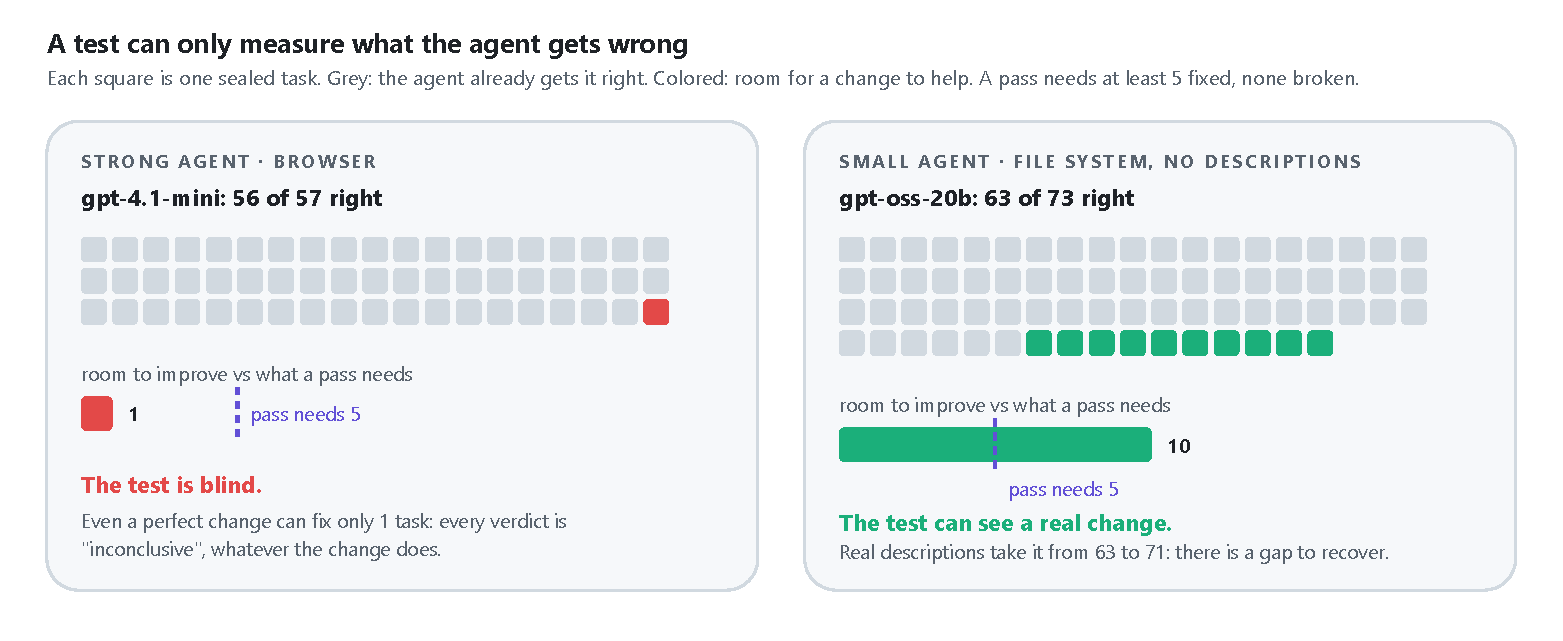
\includegraphics[width=\linewidth]{figures/ceiling.pdf}
  \caption{Headroom. Each square is a sealed task; coloured squares are tasks the agent gets wrong. A strong agent on Browser
  leaves one, so no change can reach the five fixed tasks a pass needs. A small agent on File System without descriptions
  leaves ten.}
  \label{fig:ceiling}
\end{figure}

\paragraph{Three levels of correctness.} We report, for every baseline, exact-name accuracy (the benchmark's usual metric),
equivalent-name accuracy, and executable accuracy (the gate's $c$). The gaps between them turned out to be the most important
finding of the evaluation.

\paragraph{Known-answer controls.} Each domain judges overlays whose verdict is known: a \emph{harmful route} from the tool
serving the most baseline-correct tasks to an argument-compatible tool that is not acceptable for them (must \fail, and the
harness predicts the exact number of broken tasks), and an \emph{empty overlay} (must be \incon).

\paragraph{Undocumented servers.} Many real servers ship terse or missing descriptions. In the \emph{no-descriptions} condition
every tool keeps its name and schema but loses its description. This gives the loop a deficit with a known remedy, and a third
control, \emph{restore}, puts the real descriptions back.

\section{Results}\label{sec:results}

\begin{table}[t]
\centering\small
\caption{\texttt{gpt-4.1-mini}, servers with their real descriptions. Sealed-set baseline under three correctness levels, improver result on DEV and the
gate's verdict on SEALED. $^\dagger$This run's harmful control routed to an equivalent twin and broke nothing (corrected in
Table~\ref{tab:nodocs}). $^\ddagger$No argument-compatible route exists.}
\label{tab:full}
\begin{tabular}{lrcccc}
\toprule
Domain & $|T|$ & exact / equiv.\ / exec. & DEV & SEALED verdict & Harmful \\
\midrule
Browser     & 57  & 38 / 56 / 56  & 123$\to$126 & \incon{} (out of reach) & --$^\dagger$ \\
Map         & 150 & 52 / 121 / 121 & no gain    & --                & --$^\dagger$ \\
Pay         & 93  & 86 / 86 / 86  & no gain     & --                & --$^\ddagger$ \\
Search      & 55  & 42 / 54 / 53  & no gain     & --                & \fail, 11 \\
File System & 73  & 64 / 64 / 64  & 147$\to$149 & \incon{} (64$\to$64) & \fail, 14 \\
\bottomrule
\end{tabular}
\end{table}

\begin{table}[t]
\centering\small
\caption{\texttt{gpt-4.1-mini}, servers without descriptions. Headroom is the number of sealed tasks the baseline gets wrong; a pass needs at least 5
fixed with none broken. Harmful: verdict, broken tasks (predicted). Empty controls were \incon{} in all five domains.}
\label{tab:nodocs}
\begin{tabular}{lcccccc}
\toprule
Domain & Baseline & Headroom & DEV & Candidate on SEALED & Harmful & Restore real docs \\
\midrule
Map         & 105/150 & 45 & 268$\to$288 & \pass{}: \textbf{+17, $-$0} & \fail, 6 (6)  & \fail: +15, $-$2 \\
File System & 64/73   & 9  & 145$\to$149 & \incon{} (64$\to$64)       & \fail, 14 (14) & \incon \\
Pay         & 89/93   & 4  & no gain     & --                         & --             & \fail: $-$1 \\
Search      & 54/55   & 1  & no gain     & --                         & \fail, 11 (11) & \incon \\
Browser     & 56/57   & 1  & no gain     & --                         & \fail, 6 (6)   & \incon \\
\bottomrule
\end{tabular}
\end{table}

\begin{figure}[t]
  \centering
  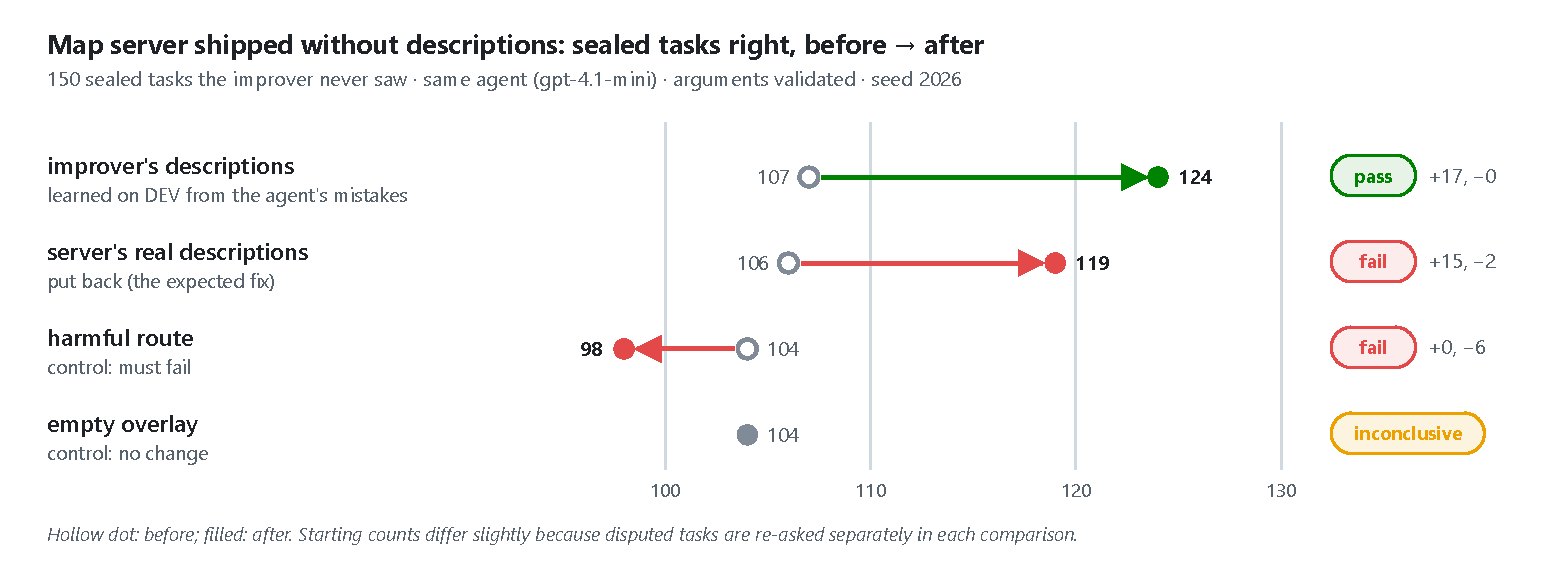
\includegraphics[width=\linewidth]{figures/results.pdf}
  \caption{Map without descriptions: sealed tasks correct before (hollow) and after (filled) each overlay, with the gate's
  verdict. Starting counts differ slightly because disputed tasks are re-asked separately per comparison.}
  \label{fig:results}
\end{figure}

\paragraph{The gate behaves as designed.} Harmful controls failed with exactly the predicted number of broken tasks in every domain
where one exists (Table~\ref{tab:nodocs}); empty controls were \incon{} in all domains.

\paragraph{Equivalence dominates the apparent error.} On Map, exact-name accuracy is 52/150 but executable accuracy is
121/150 (Table~\ref{tab:full}): most ``mistakes'' are the same action on a sibling server, which the dataset itself lists as
equivalent. With equivalents counted, Browser and Search have one or two sealed errors left, so no candidate could pass there.

\paragraph{A real, executable improvement.} On Map without descriptions the loop's candidate fixed 17 sealed tasks and broke none
(Figure~\ref{fig:results}). The learned descriptions state general rules (``use this when you have coordinates and want the
address''), name the neighbouring tool to use instead, use the parameter names, and copy no DEV request. They outperform the
server's own descriptions, which fixed 15 but broke 2 and are therefore failed by the zero-regression rule. Pruning was necessary:
each full proposal scored below the DEV baseline (239, 246 and 250 of 346 against 268), each pruned one above it (271, 260, 288).

\paragraph{Whether descriptions matter depends on the agent.} Without any descriptions, \texttt{gpt-4.1-mini} scores the same on
Browser, Search and File System, and higher on Pay (89 vs 86 of 93): it chooses mostly from tool names and schemas. This, rather
than a weak improver, explains why the documented servers yielded nothing to ship. The gpt-oss agents behave differently
(Table~\ref{tab:oss}, Figure~\ref{fig:models}): on the same 73 File System tasks, removing descriptions costs \texttt{gpt-oss-20b}
8 tasks and \texttt{gpt-oss-120b} 6. Size is not the explanation: the larger gpt-oss model scores below the smaller one with the
real descriptions (69 vs 71). With their descriptions both gpt-oss agents leave fewer than 5 sealed errors (a blind test); without
them both miss 10, a gap with a known remedy and the setting in which the loop is meant to work.

\begin{table}[t]
\centering\small
\caption{Primary testbed, File System, 73 sealed tasks, executable correctness. Headroom is the number of sealed tasks the
baseline gets wrong.}
\label{tab:oss}
\begin{tabular}{lcccc}
\toprule
Agent & Real descriptions & No descriptions & Descriptions worth & Headroom (with / without) \\
\midrule
\texttt{gpt-oss-20b}  & \textbf{71} & 63 & 8 & 2 / 10 \\
\texttt{gpt-oss-120b} & 69          & 63 & 6 & 4 / 10 \\
\texttt{gpt-4.1-mini} & 64          & 64 & 0 & 9 / 9 \\
\bottomrule
\end{tabular}
\end{table}

\begin{figure}[t]
  \centering
  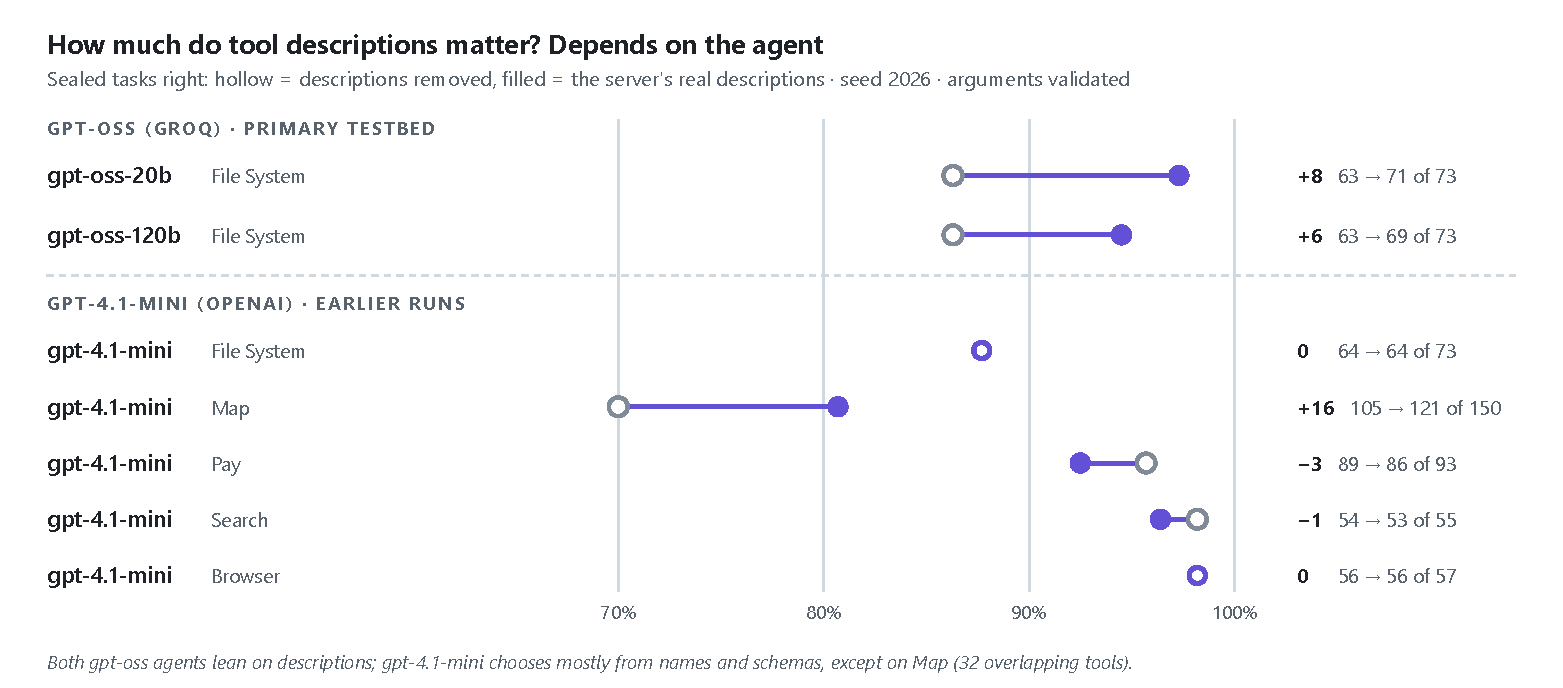
\includegraphics[width=\linewidth]{figures/models.pdf}
  \caption{Sealed tasks right with the server's real descriptions (filled) and with descriptions removed (hollow), by agent and
  domain.}
  \label{fig:models}
\end{figure}

\paragraph{The primary-testbed loop is not finished.} A reduced no-descriptions run (200 tasks, 60 sealed, 2 improver rounds,
controls skipped) measured the sealed baseline at 54/60 and was then stopped, as designed, by the provider's free-tier daily token
limit during the improver's first DEV pass. The full run needs roughly $9\times10^5$ agent tokens. Its result is the most important
open measurement of this work.

\section{What we got wrong}\label{sec:lessons}

The evaluation was corrected several times, and the corrections are the most transferable result.
\begin{itemize}
  \item \textbf{Name-only scoring produced a fake gain.} An earlier result of +8.6 points on File System (four seeds, confidence
  interval above zero) came entirely from routing \texttt{read\_text\_file} to \texttt{read\_multiple\_files}. Scored by tool name it
  looked right; a real call through the proxy failed because the target expects \texttt{paths}, not \texttt{path}. As a
  description-only change the same fix fixed 0 of 73 tasks.
  \item \textbf{Label noise looked like room to improve.} Most errors on Map, Browser and Search were equivalent tools; an earlier
  route that ``fixed'' Browser was steering the agent toward the labeler's arbitrary choice.
  \item \textbf{Majority voting was not enough.} An identical overlay was failed because a task the model answers right about half
  the time disagrees with itself about half the time; the decisive-flip rule fixed it.
  \item \textbf{A control can rot.} Once equivalents counted, the harmful control routed to a twin and broke nothing. A control
  must predict its own effect size.
  \item \textbf{A gate that never passes proves nothing.} Until the no-descriptions condition, the gate had only ever said \fail{}
  or \incon; it was indistinguishable from a gate that blocks everything.
  \item \textbf{Infrastructure failures masquerade as agent errors.} When API credits ran out mid-run, every call failed and would
  have been recorded as agent mistakes; fatal API errors now stop the run.
\end{itemize}

\section{Limitations}

The positive result rests on one domain, one seed and one agent model (\texttt{gpt-4.1-mini}); a second seed was blocked by API
quota, and the full loop on the primary testbed was stopped by a free-tier daily limit. The agent is a
single-call stand-in for production agents in multi-step sessions, and some remaining Map ``errors'' (geocoding before asking
for directions) are plausible first steps scored against a single-call label. Labels come from a benchmark; for real servers,
golden tasks are drafted from the tool documentation and approved by a person, and drafted tasks are easier than real traffic.
Except for File System, correctness is schema validity rather than execution. The no-descriptions condition is a simulation of
a common situation, not a measured deployment.

\section{Conclusion}

Self-improving tool interfaces are feasible only with a judge that is harder to fool than the improver is to write. With
executable correctness, equivalence-aware labels, decisive re-voting, fatal regressions and known-answer controls, the gate
refused every harmful and every unproven change across five domains and passed one real improvement, learned from mistakes and
validated on unseen tasks. Choosing the agent under test turned out to matter as much as the method: a strong agent leaves too
few mistakes, and may not read descriptions at all, so its results say little and do not last. The next steps are the full loop
on the primary testbed (\texttt{gpt-oss-20b} without descriptions), further seeds, real traffic in place of benchmark labels, and
multi-step tasks where a description's value is the call that follows the choice.

\appendix
\section{Reproducibility}
Code, figures and this paper: \url{https://github.com/FirePheonix/Self-Improving-MCPs}. The benchmark is run with
\texttt{sh scripts/bench/run-all.sh [seed]} (Groq and gpt-oss by default, \texttt{PROVIDER=openai} for the
\texttt{gpt-4.1-mini} runs); the no-descriptions condition with \texttt{DOCS=none}, a cheap baseline probe with
\texttt{BASELINE\_ONLY=1}. Each domain writes a log
with one machine-readable result line containing every verdict, count, candidate overlay, mistake group and improver round.

\bibliographystyle{plainnat}
\bibliography{refs}

\end{document}
